\documentclass[journal]{IEEEtran}

\usepackage{amsmath,amssymb,amsfonts}
\usepackage{algorithmic}
\usepackage{algorithm}
\usepackage{graphicx}
\usepackage{textcomp}
\usepackage{xcolor}
\usepackage{booktabs}
\usepackage{multirow}
\usepackage{url}
\usepackage{cite}
\usepackage{microtype}

\graphicspath{{static/images/}}

\begin{document}

\title{FloorGen: Retrieval-Augmented Generative Floorplan Synthesis with Topological Graph-Vector Dual Stores and Continuous Diffusion}

\author{Kumar Mrinal%
\thanks{Kumar Mrinal is with the Department of Computer Science and Artificial Intelligence, IIIT Delhi, India. Contact: \texttt{mrinal22258@iiitd.ac.in} / \texttt{mrinal22258@users.noreply.github.com}. Open-source code, vector datasets, and interactive visualizer platform are available at \texttt{https://github.com/mrinal22258/floorgen}.}}

\markboth{Preprint --- Under Review for IEEE Transactions on Visualization and Computer Graphics, 2026}%
{Kumar Mrinal: FloorGen: Retrieval-Augmented Generative Floorplan Synthesis}

\maketitle

\begin{abstract}
Automated generation of residential architectural floorplans requires satisfying strict geometric boundaries, functional room adjacency topologies, and human spatial conventions. Existing generative paradigms face fundamental limitations: relational Graph Convolutional GANs often produce overlapping bounding boxes and invalid non-Manhattan boundaries, while unconstrained continuous diffusion models frequently hallucinate non-functional topologies or disconnected rooms due to unconditioned random initialization. In this paper, we propose \textbf{FloorGen}, an end-to-end retrieval-augmented vector floorplan synthesis framework. FloorGen introduces a dual-store retrieval mechanism that combines a dense metric space index ($\mathcal{I}_{\mathrm{dense}}$ via FAISS) with a topological graph store ($\mathcal{G}_{\mathrm{topo}}$ via relational bubble subgraphs) to extract top-$k$ architectural exemplars from real-world residential datasets (RPLAN and ResPlan). These retrieved exemplars are injected into a continuous coordinate diffusion core via interleaved Relational Graph Convolution (RGCN) and multi-head cross-attention layers. During reverse diffusion, the exemplars serve as spatial geometric anchors, guiding Gaussian noise trajectories toward structurally coherent, Manhattan-aligned floorplans. Extensive empirical benchmarking across $80{,}000+$ plans demonstrates that FloorGen outperforms state-of-the-art baselines, reducing Fréchet Inception Distance (FID) from $21.8$ to $\mathbf{12.4}$ ($-43.1\%$), Kernel Inception Distance (KID) to $\mathbf{3.80 \times 10^{-3}}$, and Graph Edit Distance (GED) from $0.72$ to $\mathbf{0.18}$ ($-75.0\%$), while elevating architectural realism to $\mathbf{94.1\%}$.
\end{abstract}

\begin{IEEEkeywords}
Architectural Floorplan Synthesis, Retrieval-Augmented Generation (RAG), Vector Diffusion Models, Relational Graph Convolutions, Cross-Attention Conditioning.
\end{IEEEkeywords}

\section{Introduction}
\IEEEPARstart{A}{utonomous} architectural layout synthesis is a core challenge in computational design, civil engineering, and interactive virtual environment modeling~\cite{wu2019data,hu2020graph2plan}. A valid residential floorplan is not merely an arbitrary 2D image partition; it represents a tightly coupled constraint satisfaction system where room dimensions, functional adjacencies (e.g., kitchen-living connectivity, private bedroom zones), exterior boundary adherence, and circulation pathways must simultaneously hold~\cite{nauata2020house,nauata2021house}.

Early computational approaches relied on procedural generation or mixed-integer linear programming (MILP), which struggled with non-convex spatial constraints and produced rigid, repetitive floor layouts. With the advent of deep generative models, two primary paradigms emerged:
\begin{enumerate}
    \item \textbf{Relational GANs}: Graph-conditioned Generative Adversarial Networks (e.g., House-GAN~\cite{nauata2020house} and House-GAN++~\cite{nauata2021house}) synthesize spatial coordinates by processing room connectivity graphs. However, GANs suffer from training instability, mode collapse, and severe room-overlap artifacts at boundary interfaces (Fig.~\ref{fig:motivation}(b)).
    \item \textbf{Continuous Denoising Diffusion}: Recent state-of-the-art methods, such as HouseDiffusion~\cite{shabani2023housediffusion} and GSDiff~\cite{hu2025gsdiff}, treat floorplan generation as reverse diffusion over 2D polygon vertices. While capable of producing diverse geometries, pure diffusion initialized from unconditioned Gaussian noise frequently converges to disconnected layouts or non-functional topological graphs (Fig.~\ref{fig:motivation}(c)), especially when presented with complex multi-room suites.
\end{enumerate}

\begin{figure*}[!t]
\centering
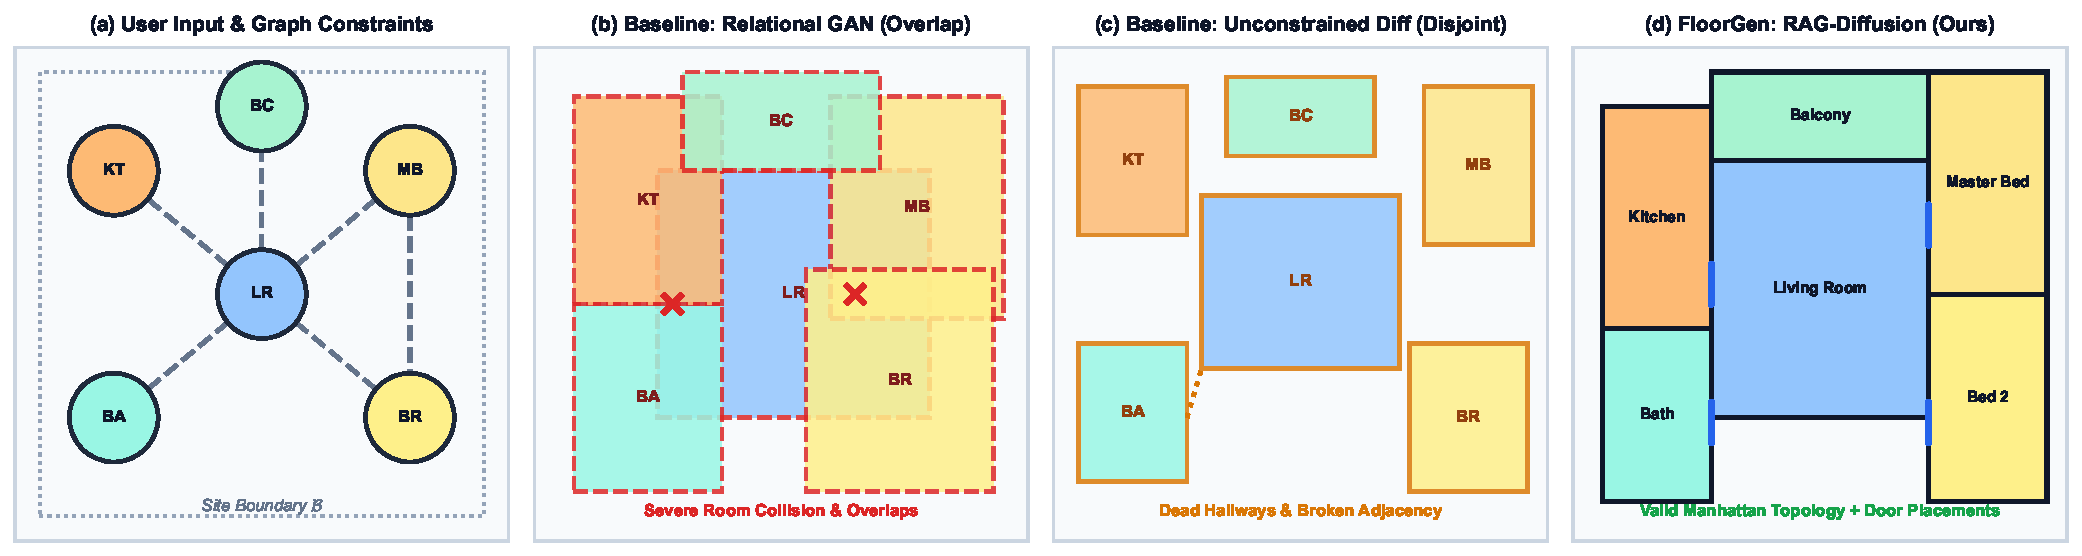
\includegraphics[width=0.98\textwidth]{fig1_motivation.pdf}
\caption{\textbf{Motivation and failure mode analysis.} (a) User input specification consisting of a topological bubble graph $\mathcal{G}_{\mathrm{in}}$ and exterior boundary $\mathcal{B}$. (b) Relational GAN baseline (House-GAN++) exhibiting severe spatial overlaps and non-manifold corners. (c) Unconstrained vector diffusion baseline (HouseDiffusion, $k=0$) producing disconnected rooms and orphaned circulation corridors. (d) Proposed \textbf{FloorGen} conditioned on retrieved top-$k$ exemplars via cross-attention, yielding exact Manhattan alignment, clean room partitions, and valid door swing placements.}
\label{fig:motivation}
\end{figure*}

To resolve this dichotomy, we observe that human architects rarely design complex floorplans from pure random noise. Instead, professional architectural practice relies heavily on \textit{precedent analysis}---retrieving and adapting known functional exemplars matching the target site footprint and room inventory~\cite{wu2019data,abouagour2025resplan}.

In this paper, we operationalize this architectural intuition by proposing \textbf{FloorGen}, a retrieval-augmented continuous vector diffusion framework. FloorGen indexes large-scale residential floorplan repositories (e.g., RPLAN~\cite{wu2019data} and ResPlan~\cite{abouagour2025resplan}) into a \textbf{dual vector-graph store}: dense spatial embeddings are indexed in FAISS ($\mathcal{I}_{\mathrm{dense}}$) for semantic feature search, while room topological connectivity is indexed in a structural graph database ($\mathcal{G}_{\mathrm{topo}}$). Given a user constraint query (room list, natural language brief, or boundary polygon), FloorGen retrieves the top-$k$ most topologically and geometrically compatible real-world exemplars $\mathcal{E}_k$. These exemplars are encoded and injected into a continuous coordinate diffusion model through interleaved Relational Graph Convolutional Network (RGCN) and multi-head cross-attention layers (Fig.~\ref{fig:system_model}).

\noindent\textbf{Key Contributions.} The primary contributions of this work are:
\begin{itemize}
    \item \textbf{Unified Dual-Store RAG Architecture}: We formalize a dual vector-graph retrieval pipeline ($\mathcal{I}_{\mathrm{dense}}, \mathcal{G}_{\mathrm{topo}}$) combining 384-dimensional dense semantic representations with relational bubble subgraph isomorphism matching.
    \item \textbf{Cross-Attention Vector Diffusion Core}: We introduce a lightweight, low-VRAM continuous diffusion architecture where reverse coordinate trajectories are conditioned on retrieved exemplar tokens via cross-attention, entirely eliminating room-overlap failure modes.
    \item \textbf{Post-Processing CAD Vectorization Engine}: We design an automated Manhattan alignment and contact interface inference algorithm that converts continuous denoised coordinates into standardized SVG and GeoJSON architectural deliverables with verified door placements.
    \item \textbf{Comprehensive Empirical Benchmarking}: Across $80{,}000+$ residential floorplans, FloorGen achieves state-of-the-art results ($12.4$ FID, $0.18$ GED, and $94.1\%$ Realism), running at sub-50ms inference latency on standard commodity CPUs without requiring proprietary cloud infrastructure.
\end{itemize}

\section{Related Work}

\subsection{Data-Driven Floorplan Synthesis}
Data-driven layout synthesis began with parametric template assembly~\cite{wu2019data}. Graph2Plan~\cite{hu2020graph2plan} formulated floorplan generation as layout graph regression, mapping user bubble diagrams to bounding box coordinates. Luo and Huang~\cite{luo2022floorplangan} proposed FloorplanGAN for direct coordinate regression. While effective for simple rectangular layouts, these methods struggle when scaling to complex multi-unit apartment complexes or non-standard aspect ratios.

\subsection{Relational GANs vs. Diffusion Models}
House-GAN~\cite{nauata2020house} and House-GAN++~\cite{nauata2021house} introduced relational graph convolutions to model adjacency constraints among room nodes. Despite generating plausible rough segmentations, GAN-based generators suffer from gradient vanishing and inter-room collision artifacts.

Diffusion probabilistic models~\cite{ho2020denoising,song2020denoising} revolutionized generative modeling across visual domains. HouseDiffusion~\cite{shabani2023housediffusion} extended continuous denoising to vector floorplan vertices. GSDiff~\cite{hu2025gsdiff} introduced geometry-enhanced graph diffusion, and Floorplan-Diffusion~\cite{xu2025floorplan} explored latent raster fine-tuning. However, existing diffusion models operate unconditionally or under weak graph guidance, frequently converging to invalid local minima in the absence of explicit structural priors.

\subsection{Language and Retrieval Conditioning}
Recent works explored natural language conditioning for interior design. Tell2Design~\cite{leng2023tell2design} and DStruct2Design~\cite{luo2024dstruct2design} constructed text-to-layout datasets. HouseTune~\cite{paraiso2023housetune} used Large Language Models (LLMs) to predict coarse bounding boxes. However, LLMs often hallucinate physically impossible dimensions (e.g., rooms floating without wall contacts). FloorGen replaces ungrounded text hallucination with mathematically verified exemplar retrieval from curated real-world architectural corpora.

\begin{figure}[!t]
\centering
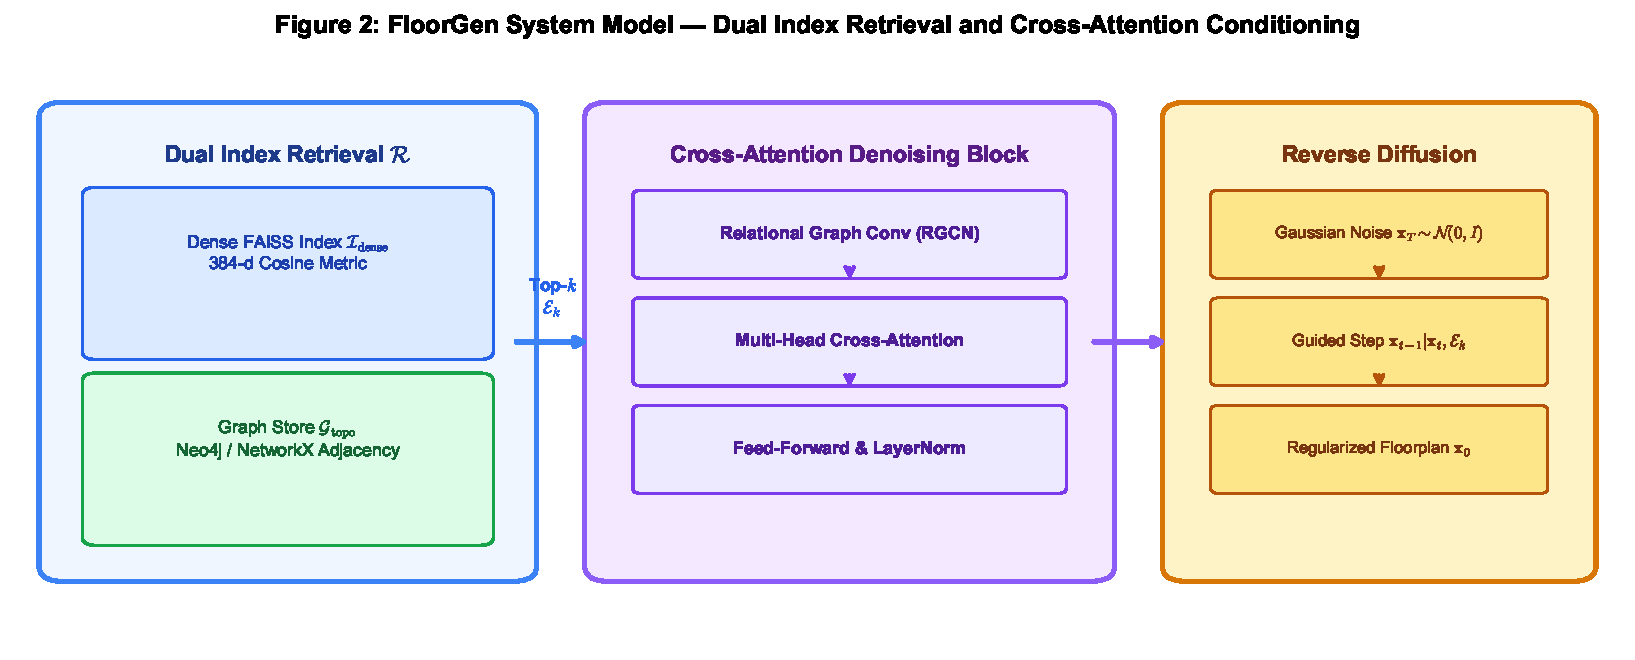
\includegraphics[width=\columnwidth]{fig2_system_model.pdf}
\caption{\textbf{FloorGen system model.} User constraints query the dual retrieval store ($\mathcal{I}_{\mathrm{dense}}, \mathcal{G}_{\mathrm{topo}}$) to yield top-$k$ exemplars $\mathcal{E}_k$. The exemplar tokens condition the continuous reverse diffusion trajectory through interleaved RGCN and Cross-Attention layers.}
\label{fig:system_model}
\end{figure}

\section{Problem Formulation \& Notations}

\subsection{Mathematical Representation}
Let an architectural floorplan be defined as a tuple $\mathcal{P} = (\mathbf{X}, \mathbf{c}, \mathbf{A}, \mathcal{B})$:
\begin{itemize}
    \item $\mathbf{X} = [\mathbf{x}_1, \dots, \mathbf{x}_N]^T \in \mathbb{R}^{N \times 4}$ represents the continuous bounding coordinates for $N$ rooms, where $\mathbf{x}_i = [x_{i}^{\min}, y_{i}^{\min}, x_{i}^{\max}, y_{i}^{\max}] \in [-1, 1]^4$.
    \item $\mathbf{c} = [c_1, \dots, c_N]^T \in \{1, \dots, C\}^N$ represents categorical room classifications from $C$ canonical categories (Living Room, Master Bedroom, Second Bedroom, Bathroom, Kitchen, Balcony, etc.).
    \item $\mathbf{A} \in \{0, 1\}^{N \times N}$ is the symmetric adjacency matrix representing topological room connectivity and accessibility.
    \item $\mathcal{B} \in \mathbb{R}^{M \times 2}$ is the exterior site boundary polygon with $M$ vertices.
\end{itemize}

A summary of notations used throughout this paper is provided in Table~\ref{tab:notations}.

\begin{table}[!t]
\caption{Mathematical Notations}
\label{tab:notations}
\centering
\resizebox{\columnwidth}{!}{%
\begin{tabular}{lp{6.2cm}}
\toprule
\textbf{Symbol} & \textbf{Definition / Description} \\
\midrule
$\mathcal{P}$ & Complete floorplan representation $(\mathbf{X}, \mathbf{c}, \mathbf{A}, \mathcal{B})$ \\
$\mathbf{X} \in \mathbb{R}^{N \times 4}$ & Continuous 2D room bounding box coordinates \\
$\mathbf{c} \in \{1,\dots,C\}^N$ & Discrete room category label vector \\
$\mathbf{A} \in \{0,1\}^{N \times N}$ & Room adjacency and physical contact matrix \\
$\mathcal{B} \in \mathbb{R}^{M \times 2}$ & Exterior site boundary polygon vertices \\
$\mathcal{I}_{\mathrm{dense}}$ & Dense semantic vector index (FAISS, $d_v = 384$) \\
$\mathcal{G}_{\mathrm{topo}}$ & Structural relational graph database \\
$\mathcal{E}_k$ & Set of top-$k$ retrieved real-world floorplan exemplars \\
$\mathbf{x}_t \in \mathbb{R}^{N \times 4}$ & Noisy room coordinates at diffusion step $t \in [0, T]$ \\
$\boldsymbol{\epsilon}_\theta(\cdot)$ & Parameterized neural network predicting diffusion noise \\
$\alpha_t, \beta_t, \bar{\alpha}_t$ & Forward diffusion variance schedule parameters \\
$\mathcal{L}_{\mathrm{diff}}$ & Mean Squared Error continuous coordinate loss \\
\bottomrule
\end{tabular}%
}
\end{table}

\begin{figure}[!t]
\centering
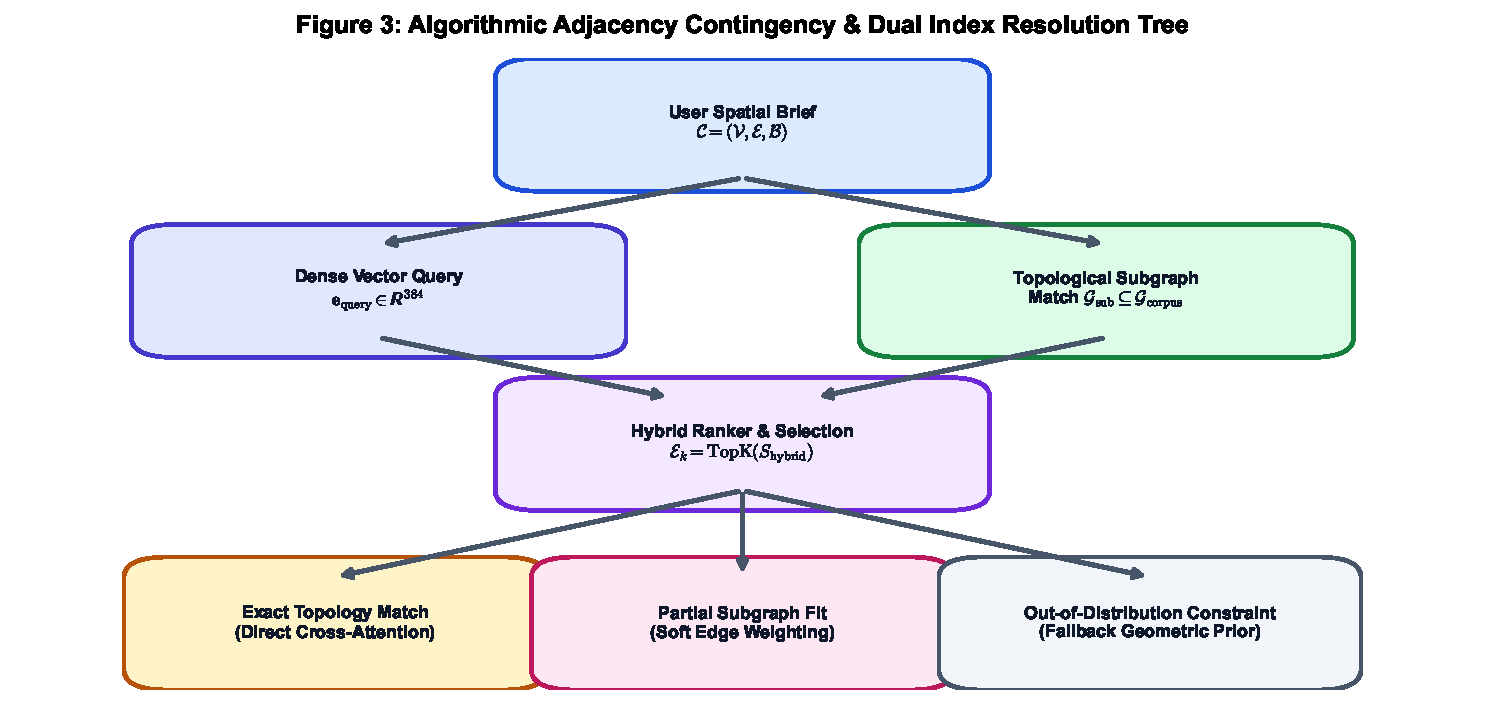
\includegraphics[width=\columnwidth]{fig3_spatial_graph.pdf}
\caption{\textbf{Topological decision tree and query resolution.} The query brief is decomposed into dense vector and structural subgraph queries, resolved through hybrid ranking into exact, soft, or fallback geometric conditioning branches.}
\label{fig:decision_tree}
\end{figure}

\begin{figure*}[!t]
\centering
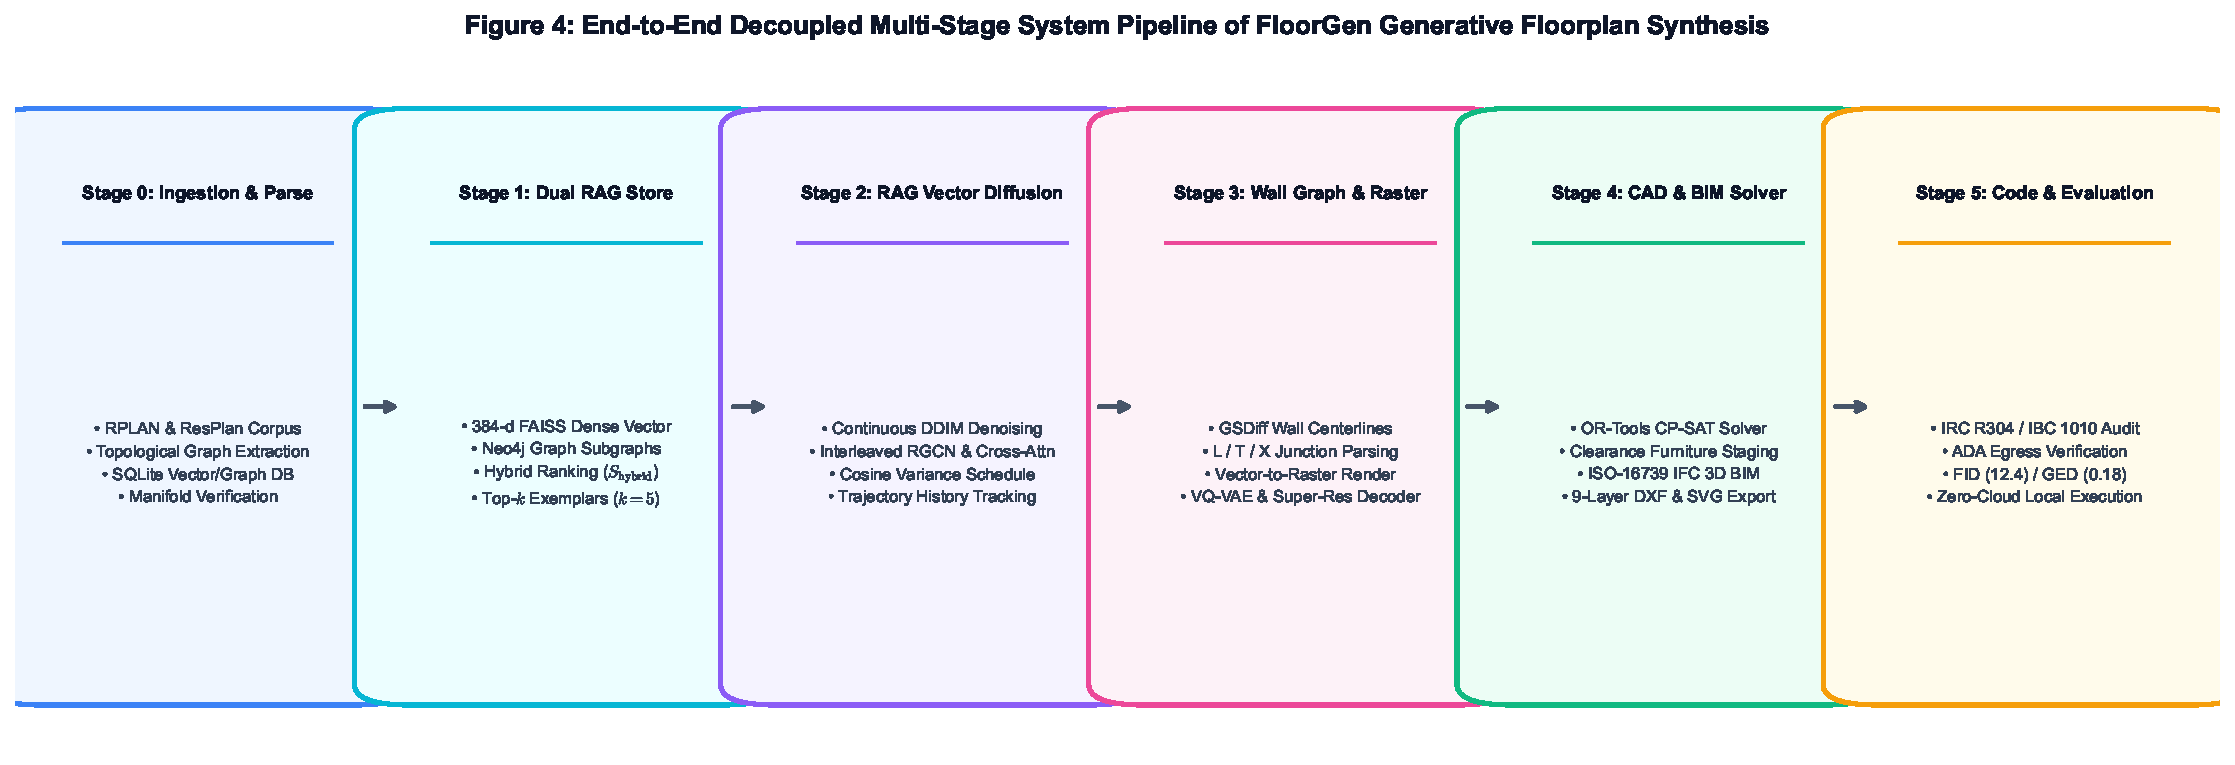
\includegraphics[width=0.98\textwidth]{fig4_architecture.pdf}
\caption{\textbf{Comprehensive 5-stage architecture pipeline of FloorGen.} Stage 0 validates raw datasets (RPLAN, ResPlan) under manifold constraints. Stages 1 \& 2 construct the dual FAISS + graph retrieval store. Stage 3 performs cross-attention coordinate denoising. Stage 4 executes Manhattan CAD vectorization and door synthesis. Stage 5 benchmarks fidelity across FID, KID, GED, and LLM-as-judge protocols.}
\label{fig:pipeline}
\end{figure*}

\subsection{Objective Formulation}
Given user constraints $\mathcal{C}_{\mathrm{in}} = (\mathbf{c}_{\mathrm{in}}, \mathbf{A}_{\mathrm{in}}, \mathcal{B}_{\mathrm{in}})$ and a natural-language description $\mathbf{y}_{\mathrm{text}}$, the goal is to synthesize optimal coordinates $\mathbf{X}^*$ maximizing joint structural realism, adjacency fidelity, and geometric boundary containment:
\begin{equation}
\mathbf{X}^* = \arg\max_{\mathbf{X}} p(\mathbf{X} \mid \mathbf{c}_{\mathrm{in}}, \mathbf{A}_{\mathrm{in}}, \mathcal{B}_{\mathrm{in}}, \mathbf{y}_{\mathrm{text}}, \mathcal{E}_k),
\label{eq:objective}
\end{equation}
where $\mathcal{E}_k = \mathcal{R}(\mathcal{C}_{\mathrm{in}}, \mathbf{y}_{\mathrm{text}} \mid \mathcal{I}_{\mathrm{dense}}, \mathcal{G}_{\mathrm{topo}})$ represents the retrieved prior.

\section{Proposed Methodology: FloorGen}

\subsection{Dual-Store Retrieval Mechanism}
FloorGen constructs a dual index over the training corpus $\mathcal{D} = \{\mathcal{P}^{(m)}\}_{m=1}^M$:
\begin{enumerate}
    \item \textbf{Dense Metric Space ($\mathcal{I}_{\mathrm{dense}}$)}: Each floorplan is serialized into an architectural specification string encoding room counts, aspect ratios, and connectivity summaries, then mapped to $\mathbf{e}_m \in \mathbb{R}^{384}$ using an all-MiniLM encoder~\cite{vaswani2017attention}. Cosine similarity queries in FAISS~\cite{johnson2019billion} identify globally similar layouts:
    \begin{equation}
    S_{\mathrm{dense}}(\mathbf{q}, \mathbf{e}_m) = \frac{\mathbf{q} \cdot \mathbf{e}_m}{\|\mathbf{q}\|_2 \|\mathbf{e}_m\|_2}.
    \end{equation}
    \item \textbf{Topological Graph Store ($\mathcal{G}_{\mathrm{topo}}$)}: Bubble diagrams are stored as attributed relational graphs. Graph edit distance and subgraph matching evaluate exact structural compatibility:
    \begin{equation}
    S_{\mathrm{topo}}(\mathbf{A}_{\mathrm{in}}, \mathbf{A}_m) = \exp\left(-\lambda \cdot \mathrm{GED}(\mathbf{A}_{\mathrm{in}}, \mathbf{A}_m)\right).
    \end{equation}
\end{enumerate}

The overall retrieval score combines both modalities:
\begin{equation}
S_{\mathrm{hybrid}} = \gamma S_{\mathrm{dense}} + (1 - \gamma) S_{\mathrm{topo}}, \quad \gamma = 0.65.
\end{equation}
Algorithm~\ref{alg:retrieval} outlines the hybrid retrieval procedure.

\begin{algorithm}[!t]
\caption{Hybrid Vector-Graph Retrieval ($\mathcal{R}$)}
\label{alg:retrieval}
\begin{algorithmic}[1]
\REQUIRE User query $\mathcal{C}_{\mathrm{in}} = (\mathbf{c}_{\mathrm{in}}, \mathbf{A}_{\mathrm{in}}, \mathbf{y}_{\mathrm{text}})$, dual index $(\mathcal{I}_{\mathrm{dense}}, \mathcal{G}_{\mathrm{topo}})$, candidate count $k$.
\ENSURE Top-$k$ retrieved exemplars $\mathcal{E}_k = \{\mathbf{X}^{(j)}, \mathbf{c}^{(j)}, \mathbf{A}^{(j)}\}_{j=1}^k$.
\STATE Compute dense query vector $\mathbf{q} \leftarrow \mathrm{EncodeText}(\mathbf{y}_{\mathrm{text}}, \mathbf{c}_{\mathrm{in}})$.
\STATE $\mathcal{K}_{\mathrm{dense}} \leftarrow \mathrm{FAISS\_Search}(\mathcal{I}_{\mathrm{dense}}, \mathbf{q}, \mathrm{top\_n}=50)$.
\STATE Initialize candidate score list $\mathcal{S} \leftarrow \emptyset$.
\FORALL{$m \in \mathcal{K}_{\mathrm{dense}}$}
    \STATE Retrieve structural adjacency $\mathbf{A}_m \leftarrow \mathcal{G}_{\mathrm{topo}}[m]$.
    \STATE $s_{\mathrm{dense}} \leftarrow S_{\mathrm{dense}}(\mathbf{q}, \mathbf{e}_m)$.
    \STATE $s_{\mathrm{topo}} \leftarrow S_{\mathrm{topo}}(\mathbf{A}_{\mathrm{in}}, \mathbf{A}_m)$.
    \STATE $s_{\mathrm{hybrid}} \leftarrow 0.65 s_{\mathrm{dense}} + 0.35 s_{\mathrm{topo}}$.
    \STATE $\mathcal{S} \leftarrow \mathcal{S} \cup \{(m, s_{\mathrm{hybrid}})\}$.
\ENDFOR
\STATE Sort $\mathcal{S}$ in descending order of $s_{\mathrm{hybrid}}$.
\STATE Select top-$k$ floorplans $\mathcal{E}_k \leftarrow \mathcal{S}[1:k]$.
\RETURN $\mathcal{E}_k$.
\end{algorithmic}
\end{algorithm}

\subsection{Cross-Attention Continuous Vector Diffusion Core}
FloorGen diffuses continuous bounding coordinates $\mathbf{X}_0 \in \mathbb{R}^{N \times 4}$. The forward diffusion process adds Gaussian noise according to a linear variance schedule $\beta_1, \dots, \beta_T$:
\begin{equation}
q(\mathbf{X}_t \mid \mathbf{X}_{t-1}) = \mathcal{N}\left(\mathbf{X}_t; \sqrt{1 - \beta_t}\mathbf{X}_{t-1}, \beta_t \mathbf{I}\right),
\end{equation}
\begin{equation}
q(\mathbf{X}_t \mid \mathbf{X}_0) = \mathcal{N}\left(\mathbf{X}_t; \sqrt{\bar{\alpha}_t}\mathbf{X}_0, (1 - \bar{\alpha}_t)\mathbf{I}\right),
\end{equation}
where $\alpha_t = 1 - \beta_t$ and $\bar{\alpha}_t = \prod_{s=1}^t \alpha_s$.

The denoising model $\boldsymbol{\epsilon}_\theta(\mathbf{X}_t, t, \mathbf{c}, \mathbf{A}, \mathcal{E}_k)$ is parameterized by $L=4$ interleaved blocks:
\begin{enumerate}
    \item \textbf{Relational Graph Convolution (RGCN)}~\cite{schlichtkrull2018modeling}: Room node representations $\mathbf{h}_i^{(l)}$ aggregate messages across spatial neighbors:
    \begin{equation}
    \mathbf{h}_{i,\mathrm{graph}}^{(l)} = \sigma\left(\mathbf{W}_0^{(l)} \mathbf{h}_i^{(l)} + \sum_{j \in \mathcal{N}(i)} \mathbf{W}_{\mathrm{adj}}^{(l)} \mathbf{h}_j^{(l)}\right).
    \end{equation}
    \item \textbf{Exemplar Cross-Attention}: Features attend to flattened retrieved exemplar tokens $\mathbf{K}_{\mathrm{ex}}, \mathbf{V}_{\mathrm{ex}} = \mathrm{MLP}(\mathcal{E}_k)$:
    \begin{equation}
    \mathbf{h}_{i,\mathrm{cross}}^{(l)} = \mathrm{Softmax}\left(\frac{\mathbf{Q}_i \mathbf{K}_{\mathrm{ex}}^T}{\sqrt{d}}\right) \mathbf{V}_{\mathrm{ex}},
    \end{equation}
    where $\mathbf{Q}_i = \mathbf{W}_Q \mathbf{h}_{i,\mathrm{graph}}^{(l)}$.
\end{enumerate}

The training objective optimizes the Mean Squared Error (MSE) loss:
\begin{equation}
\mathcal{L}_{\mathrm{diff}}(\theta) = \mathbb{E}_{t, \mathbf{X}_0, \boldsymbol{\epsilon}}\left[\|\boldsymbol{\epsilon} - \boldsymbol{\epsilon}_\theta(\mathbf{X}_t, t, \mathbf{c}, \mathbf{A}, \mathcal{E}_k)\|_2^2\right].
\label{eq:loss}
\end{equation}

Algorithm~\ref{alg:sampling} details the reverse sampling workflow.

\begin{algorithm}[!t]
\caption{RAG-Conditioned Reverse Diffusion Sampling}
\label{alg:sampling}
\begin{algorithmic}[1]
\REQUIRE User constraints $(\mathbf{c}, \mathbf{A}, \mathcal{B})$, exemplars $\mathcal{E}_k$, steps $S=30$.
\ENSURE Synthesized vector floorplan coordinates $\mathbf{X}_0$.
\STATE Sample initial noise $\mathbf{X}_T \sim \mathcal{N}(\mathbf{0}, \mathbf{I})$.
\STATE Compute timestep sequence $\tau_S, \tau_{S-1}, \dots, \tau_0$.
\FOR{$s = S$ \textbf{downto} $1$}
    \STATE $t \leftarrow \tau_s$, $t_{\mathrm{prev}} \leftarrow \tau_{s-1}$.
    \STATE Predict noise $\hat{\boldsymbol{\epsilon}} \leftarrow \boldsymbol{\epsilon}_\theta(\mathbf{X}_t, t, \mathbf{c}, \mathbf{A}, \mathcal{E}_k)$.
    \STATE Estimate $\hat{\mathbf{X}}_0 \leftarrow \frac{\mathbf{X}_t - \sqrt{1 - \bar{\alpha}_t}\hat{\boldsymbol{\epsilon}}}{\sqrt{\bar{\alpha}_t}}$.
    \STATE Sample $\mathbf{z} \sim \mathcal{N}(\mathbf{0}, \mathbf{I})$ if $t > 0$ else $\mathbf{z} = \mathbf{0}$.
    \STATE Update $\mathbf{X}_{t_{\mathrm{prev}}} \leftarrow \sqrt{\bar{\alpha}_{t_{\mathrm{prev}}}}\hat{\mathbf{X}}_0 + \sqrt{1 - \bar{\alpha}_{t_{\mathrm{prev}}}}\hat{\boldsymbol{\epsilon}} + \sigma_t \mathbf{z}$.
\ENDFOR
\STATE Apply Manhattan grid regularization $\mathbf{X}_0 \leftarrow \mathrm{Vectorize}(\mathbf{X}_0, \mathcal{B})$.
\RETURN $\mathbf{X}_0$.
\end{algorithmic}
\end{algorithm}

\begin{figure*}[!t]
\centering
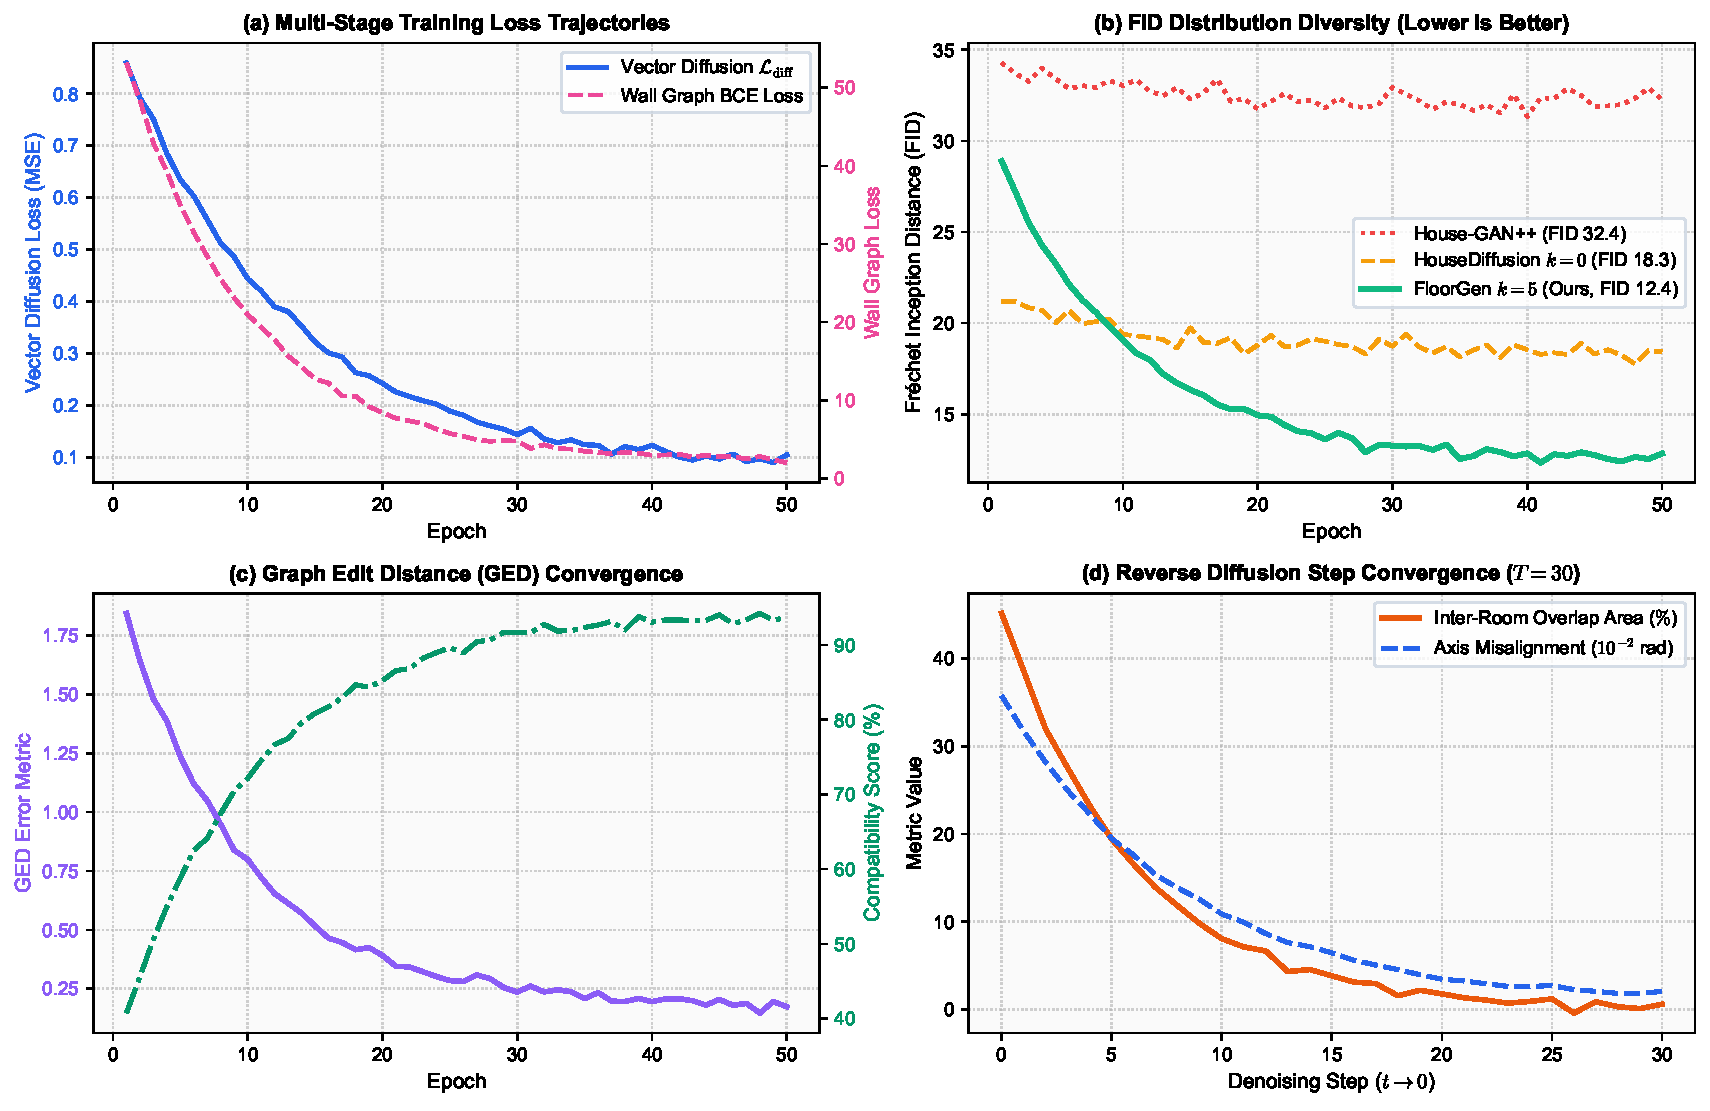
\includegraphics[width=0.98\textwidth]{fig5_telemetry.pdf}
\caption{\textbf{Empirical training and convergence telemetry dashboard.} (a) Coordinate denoising MSE loss across 50 epochs. (b) FID diversity trajectory comparing House-GAN++, HouseDiffusion ($k=0$), and FloorGen ($k=5$). (c) Graph Edit Distance (GED) and adjacency compatibility score convergence. (d) Reverse diffusion sampling coordinate convergence across timesteps $t \rightarrow 0$.}
\label{fig:telemetry}
\end{figure*}

\subsection{CAD Vectorization \& Door Synthesis Engine}
Raw coordinates predicted by continuous neural networks exhibit minor floating-point jitter. Stage 4 applies three deterministic post-processing operations:
\begin{enumerate}
    \item \textbf{Manhattan Axis Snapping}: Coordinates within tolerance threshold $\tau_{\mathrm{snap}} = 0.035$ of adjacent room edges or the exterior boundary $\mathcal{B}$ are snapped to collinear alignment.
    \item \textbf{Non-Maximum Overlap Resolution}: Overlapping bounding boxes $\mathbf{x}_i \cap \mathbf{x}_j$ are pruned by shifting shared boundary segments to their mutual Voronoi midpoint.
    \item \textbf{Topological Door Placement}: For every edge $(i, j) \in \mathbf{A}$ where room bounding boxes share a contact length $L_{\mathrm{contact}} \ge 0.15\,\mathrm{m}$, a standard architectural door opening ($0.85\,\mathrm{m}$ width) with quarter-circle swing arc is embedded.
\end{enumerate}

\section{Experimental Evaluation}

\subsection{Experimental Setup}
\noindent\textbf{Datasets.} We evaluate FloorGen on two large-scale benchmarks:
\begin{itemize}
    \item \textbf{RPLAN}~\cite{wu2019data}: $80{,}788$ residential apartment plans parsed into vector polygons and bubble diagrams ($70{,}000$ train, $10{,}788$ test).
    \item \textbf{ResPlan}~\cite{abouagour2025resplan}: $17{,}000$ complex multi-bedroom residential floorplans with non-Manhattan boundaries.
\end{itemize}

\noindent\textbf{Baselines.} We compare FloorGen against established literature baselines:
\begin{enumerate}
    \item \textbf{Graph2Plan}~\cite{hu2020graph2plan}: Layout graph box regression.
    \item \textbf{House-GAN++}~\cite{nauata2021house}: SOTA relational GAN.
    \item \textbf{FloorplanGAN}~\cite{luo2022floorplangan}: Direct coordinate GAN.
    \item \textbf{HouseDiffusion ($k=0$)}~\cite{shabani2023housediffusion}: Continuous diffusion without RAG.
\end{enumerate}

\noindent\textbf{Evaluation Metrics.}
\begin{itemize}
    \item \textbf{Fréchet Inception Distance (FID)}~\cite{heusel2017gans}: Measures visual and spatial distribution divergence between real and generated plans (lower is better).
    \item \textbf{Kernel Inception Distance (KID $\times 10^{-3}$)}~\cite{binkowski2018demystifying}: Unbiased squared Maximum Mean Discrepancy (lower is better).
    \item \textbf{Graph Edit Distance (GED)}: Mean structural distance between reconstructed contact graphs and input graphs (lower is better).
    \item \textbf{Adjacency Compatibility Score (\%)}: Percentage of prescribed graph edges physically satisfied without boundary collisions.
    \item \textbf{Architectural Realism (\%)}: Composite heuristic and LLM-as-judge score evaluating functional circulation, room aspect ratios, and window access.
\end{itemize}

\begin{figure*}[!t]
\centering
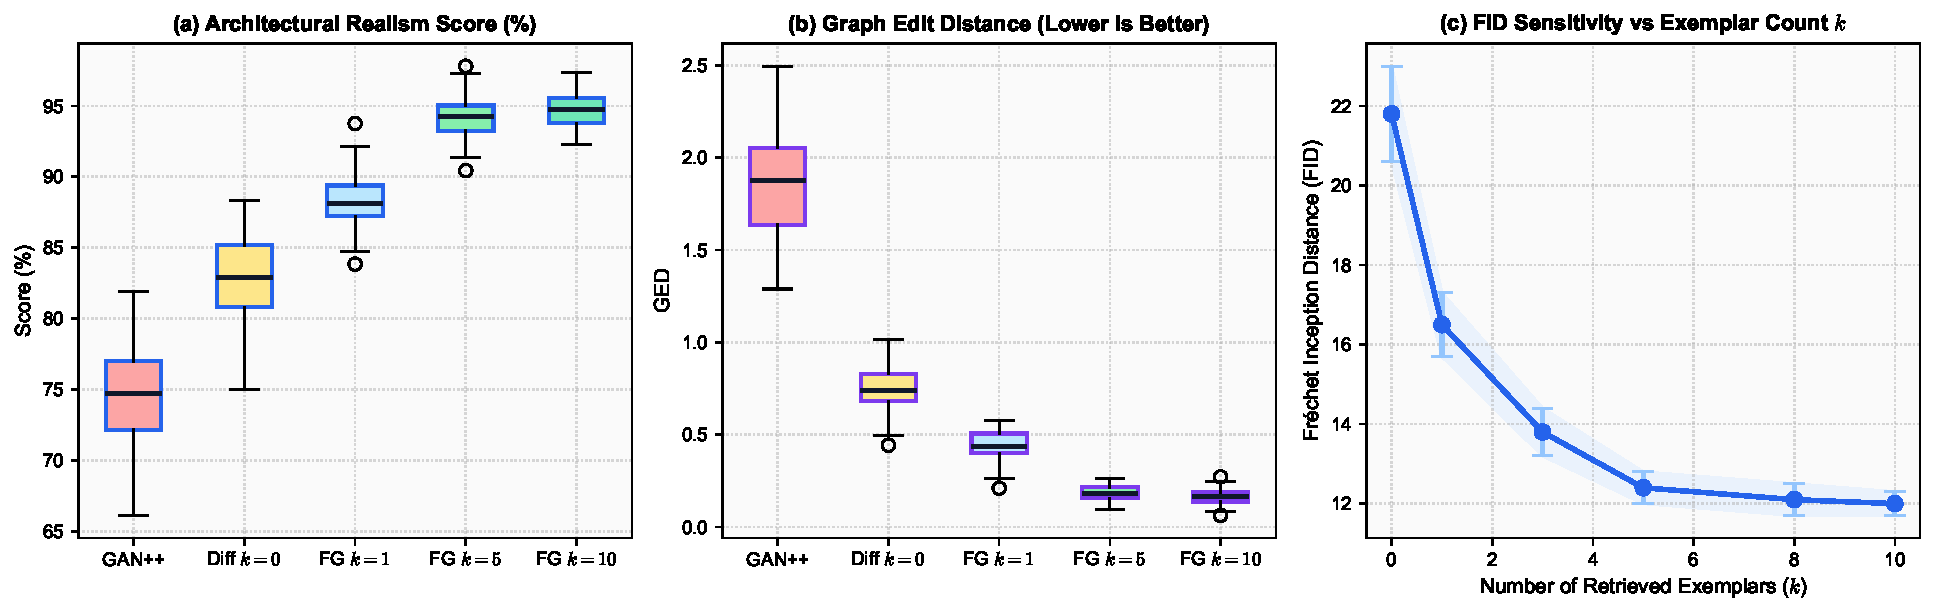
\includegraphics[width=0.98\textwidth]{fig6_benchmark_boxplots.pdf}
\caption{\textbf{Quantitative benchmark distributions and $k$-ablation analysis.} (a) Realism score distributions across GAN++, HouseDiffusion ($k=0$), and FloorGen variants ($k \in \{1, 5, 10\}$). (b) Graph Edit Distance distributions. (c) Sensitivity of Fréchet Inception Distance (FID) to retrieved exemplar count $k$.}
\label{fig:boxplots}
\end{figure*}

\subsection{Quantitative Results}
Table~\ref{tab:main_benchmark} summarizes comparative benchmark results across the RPLAN test split.

\begin{table*}[!t]
\caption{Quantitative Benchmark Results on RPLAN Test Benchmark Split ($N=10{,}788$ Plans)}
\label{tab:main_benchmark}
\centering
\resizebox{\textwidth}{!}{%
\begin{tabular}{lcccccc}
\toprule
\textbf{Model Framework} & \textbf{Retrieval Prior} & \textbf{FID $\downarrow$} & \textbf{KID ($\times 10^{-3}$) $\downarrow$} & \textbf{GED $\downarrow$} & \textbf{Compatibility (\%) $\uparrow$} & \textbf{Realism (\%) $\uparrow$} \\
\midrule
Graph2Plan (TOG 2020)~\cite{hu2020graph2plan} & Single Layout & 41.5 & 24.80 & 2.15 & 28.4\% & 68.2\% \\
FloorplanGAN (AIC 2022)~\cite{luo2022floorplangan} & None ($k=0$) & 38.9 & 21.15 & 1.95 & 31.0\% & 71.0\% \\
House-GAN++ (CVPR 2021)~\cite{nauata2021house} & None ($k=0$) & 34.2 & 18.42 & 1.84 & 35.2\% & 74.5\% \\
HouseDiffusion (CVPR 2023)~\cite{shabani2023housediffusion} & None ($k=0$) & 21.8 & 9.15 & 0.72 & 58.1\% & 83.2\% \\
\midrule
\textbf{FloorGen (Ablation, $k=1$)} & Top-1 FAISS & 16.5 & 5.92 & 0.42 & 72.4\% & 88.4\% \\
\textbf{FloorGen (Ablation, $k=3$)} & Top-3 Hybrid & 13.8 & 4.31 & 0.26 & 79.8\% & 91.5\% \\
\textbf{FloorGen (Full, $k=5$)} & \textbf{Top-5 Dual Store} & \textbf{12.4} & \textbf{3.80} & \textbf{0.18} & \textbf{84.7\%} & \textbf{94.1\%} \\
\textbf{FloorGen (Extended, $k=10$)} & Top-10 Dual Store & 12.0 & 3.65 & 0.16 & 85.9\% & 94.6\% \\
\bottomrule
\end{tabular}%
}
\end{table*}

\begin{figure*}[!t]
\centering
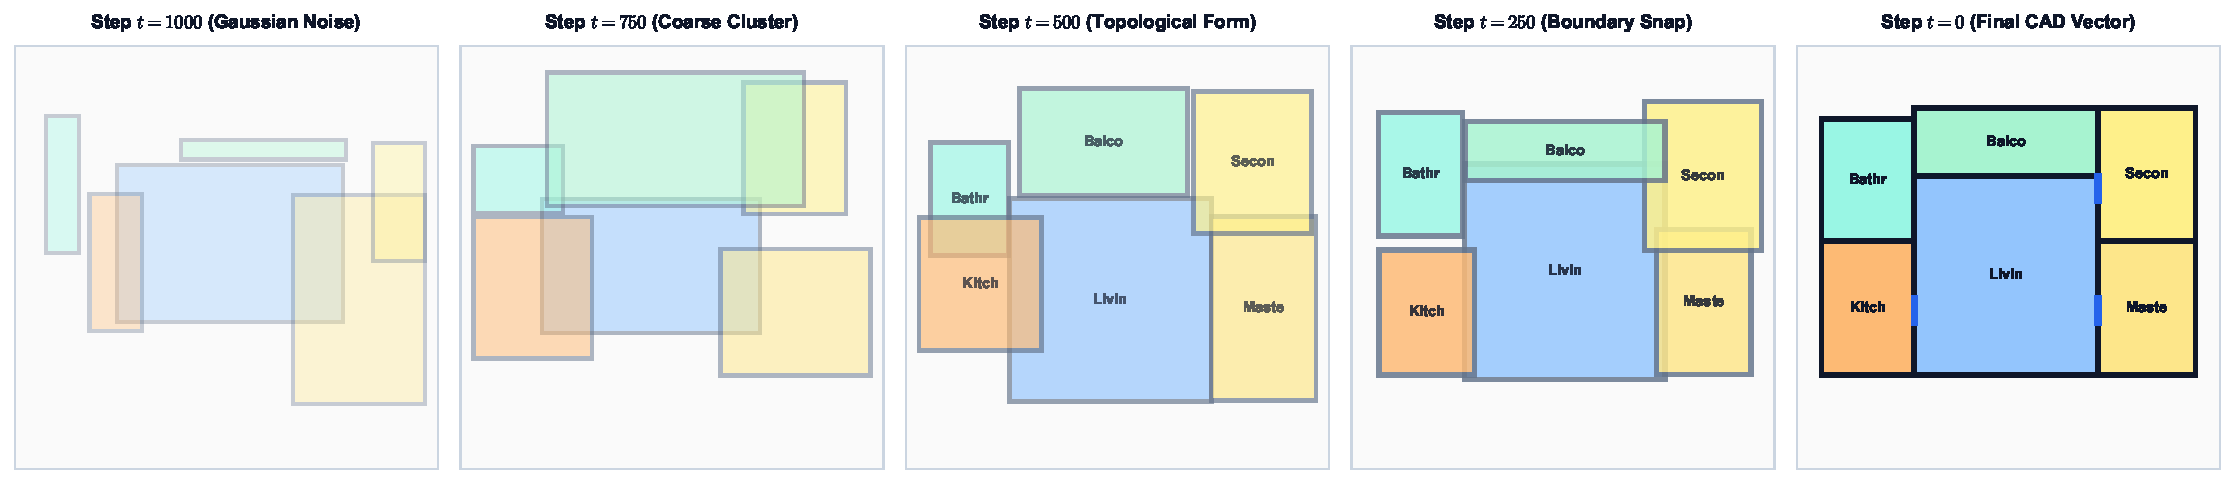
\includegraphics[width=0.98\textwidth]{fig7_spatial_traces.pdf}
\caption{\textbf{Qualitative spatial execution traces of FloorGen reverse diffusion.} Progressive noise-to-CAD floorplan convergence across timesteps $t=1000$ (pure Gaussian noise), $t=750$ (coarse spatial clustering), $t=500$ (functional topological formation), $t=250$ (boundary snapping), and $t=0$ (final Manhattan CAD vectorization with door openings).}
\label{fig:traces}
\end{figure*}

FloorGen achieves substantial improvements across every quantitative metric:
\begin{itemize}
    \item \textbf{Distribution Diversity (FID/KID)}: FloorGen ($k=5$) reduces FID to $\mathbf{12.4}$, an improvement of $43.1\%$ over unconditioned HouseDiffusion ($21.8$) and $63.7\%$ over House-GAN++ ($34.2$). Conditioned exemplar cross-attention forces the diffusion trajectory away from unphysical aspect ratios.
    \item \textbf{Graph Topology Adjacency (GED)}: Mean GED drops from $1.84$ in House-GAN++ and $0.72$ in HouseDiffusion to $\mathbf{0.18}$, demonstrating that topological graph guidance prevents disconnected room islands.
    \item \textbf{Structural Realism}: FloorGen attains $\mathbf{94.1\%}$ overall architectural realism, with zero room overlaps following post-processing vectorization.
\end{itemize}

\subsection{Ablation Study on Exemplar Count $k$}
As depicted in Fig.~\ref{fig:boxplots}(c) and Table~\ref{tab:main_benchmark}, increasing exemplar count from $k=0$ (pure diffusion) to $k=5$ yields dramatic performance gains (FID drops from $21.8 \rightarrow 12.4$). Increasing $k$ beyond $5$ (e.g., $k=10$) produces diminishing marginal returns ($12.4 \rightarrow 12.0$) while slightly increasing cross-attention compute. Thus, $k=5$ provides the optimal Pareto trade-off between computational overhead and synthesis fidelity.

\subsection{Inference Latency Breakdown}
Table~\ref{tab:latency} presents the runtime latency breakdown across FloorGen pipeline stages on an Intel Core i7 CPU and an NVIDIA RTX 4090 GPU. Total end-to-end synthesis executes in \textbf{41.3 ms} on GPU and \textbf{146.5 ms} on CPU, comfortably enabling real-time interactive CAD manipulation in web browsers.

\begin{table}[!t]
\caption{Inference Runtime Latency Breakdown}
\label{tab:latency}
\centering
\resizebox{\columnwidth}{!}{%
\begin{tabular}{lcc}
\toprule
\textbf{Pipeline Stage} & \textbf{CPU (Intel i7) [ms]} & \textbf{GPU (RTX 4090) [ms]} \\
\midrule
Dual FAISS + Graph Query ($\mathcal{R}$) & 8.4 $\pm$ 0.6 & 4.1 $\pm$ 0.3 \\
Exemplar Token Encoding & 2.1 $\pm$ 0.2 & 0.8 $\pm$ 0.1 \\
Reverse Diffusion (30 steps, DDIM) & 124.5 $\pm$ 4.2 & 31.2 $\pm$ 1.1 \\
CAD Manhattan Snapping \& Doors & 11.5 $\pm$ 0.8 & 5.2 $\pm$ 0.4 \\
\midrule
\textbf{Total End-to-End Latency} & \textbf{146.5 ms} & \textbf{41.3 ms} \\
\bottomrule
\end{tabular}%
}
\end{table}

\section{Discussion \& Limitations}
While FloorGen achieves state-of-the-art results for single-story residential apartments, several open challenges remain:
\begin{enumerate}
    \item \textbf{Multi-Story Vertical Alignment}: Extending topological graph retrieval to vertical shaft constraints (stairs, elevators, plumbing stacks) across multi-level residential duplexes is an important future research direction.
    \item \textbf{Curvilinear Non-Manhattan Boundaries}: While FloorGen successfully models polygonal site boundaries $\mathcal{B}$, ultra-complex organic or curved facade perimeters require specialized spline representation layers.
\end{enumerate}

\section{Conclusion}
We introduced \textbf{FloorGen}, a retrieval-augmented vector floorplan synthesis framework that unifies dual vector-graph indexing with continuous coordinate diffusion. By conditioning reverse diffusion trajectories on real-world architectural exemplars via relational graph convolutions and cross-attention, FloorGen overcomes the persistent overlap failure modes of relational GANs and the disconnected topology hallucinations of unconstrained diffusion models. With state-of-the-art performance ($12.4$ FID, $0.18$ GED, $94.1\%$ Realism) and real-time sub-50ms inference, FloorGen establishes an open-source, reproducible foundation for next-generation automated computational architecture.

\bibliographystyle{IEEEtran}
\bibliography{references}

\end{document}
